\documentclass{article}
\newcommand{\BEAS}{\begin{eqnarray*}}
\newcommand{\EEAS}{\end{eqnarray*}}
\newcommand{\BEAN}{\begin{eqnarray}}
\newcommand{\EEAN}{\end{eqnarray}}
\newcommand{\BEQ}{\begin{equation}}
\newcommand{\EEQ}{\end{equation}}
\newcommand{\BIT}{\begin{itemize}}
\newcommand{\EIT}{\end{itemize}}

\newcommand{\eg}{{\it e.g.\ }}
\newcommand{\ie}{{\it i.e.\ }}

\newcommand{\ones}{\mathbf 1}
\newcommand{\zeros}{\mathbf 0}
\newcommand{\reals}{{\mbox{\bf R}}}
\newcommand{\integers}{{\mbox{\bf Z}}}
\newcommand{\symm}{{\mbox{\bf S}}}  % symmetric matrices

\newcommand{\nullspace}{{\mathcal N}}
\newcommand{\range}{{\mathcal R}}
\newcommand{\Rank}{\mathop{\bf Rank}}
\newcommand{\Tr}{\mathop{\bf Tr}}

\newcommand{\sign}[1]{\mathop{\textrm{sgn}}(#1)}
\newcommand{\lambdamax}{{\lambda_{\rm max}}}
\newcommand{\lambdamin}{\lambda_{\rm min}}

\newcommand{\EE}{\mathop{\textrm{E}}}
\newcommand{\Cov}{\mathop{\textrm{Cov}}}
\newcommand{\Prob}{\mathop{\bf Prob}}
\newcommand{\Co}{{\mathop {\bf Co}}} % convex hull
\newcommand{\dist}{\mathop{\bf dist{}}}
\newcommand{\argmin}{\mathop{\rm argmin}}
\newcommand{\argmax}{\mathop{\rm argmax}}
\newcommand{\epi}{\mathop{\bf epi}} % epigraph
\newcommand{\Vol}{\mathop{\bf vol}}
\newcommand{\dom}{\mathop{\bf dom}} % domain
\newcommand{\intr}{\mathop{\bf int}}


\newcommand{\nrm}[1]{\left\lVert#1\right\rVert}
\newcommand{\nrmo}[1]{\left\lVert#1\right\rVert_1}
\newcommand{\nrmt}[1]{\left\lVert#1\right\rVert_2}
\newcommand{\nrmnn}[1]{\left\lVert#1\right\rVert_{*}}
\newcommand{\nrmf}[1]{\left\lVert#1\right\rVert_F}

\newcommand{\myexp}[1]{\mathop{\rm exp}\left\{#1\right\}}
\newcommand{\mylog}[1]{\mathop{\rm log}\left\{#1\right\}}
\newcommand{\questions}{\begin{frame}Questions?\end{frame}}
\newcommand{\LL}{\textrm{LL}}
\newcommand{\ALL}{\textrm{ALL}}

\newcommand{\KL}{\textrm{KL}}
\newcommand{\HH}{\textrm{H}}
\newcommand{\GG}{\textrm{G}}

\newcommand{\Bound}{\textrm{B}}
\newcommand{\bb}{\mathbf{b}}
\newcommand{\aaa}{\mathbf{a}}
\newcommand{\BB}{\mathbf{B}}
\newcommand{\AAA}{\mathbf{A}}
\newcommand{\CC}{\mathbf{C}}
\newcommand{\cc}{\mathbf{c}}
\newcommand{\mm}{\mathbf{m}}
\newcommand{\MM}{\mathbf{M}}
\newcommand{\nn}{\mathrm{\bf neighbors}}
\newcommand{\pa}[1]{{\textrm{\bf pa}}\left(#1\right)}
\newcommand{\pre}[2]{\mathop{\textrm{\bf pnp}}_{#1}\left(#2\right)}
\newcommand{\logsum}{\textrm{logsum}}

\newcommand{\tth}{{\textrm{th}}}
\newcommand{\xx}{\mathbf{x}}
\newcommand{\hh}{\mathbf{h}}
\newcommand{\mmu}{\mathbf{\mu}}
\newcommand{\yy}{\mathbf{y}}
\newcommand{\zz}{\mathbf{z}}
\newcommand{\dd}{\mathbf{d}}
\newcommand{\new}{\textrm{new}}
\newcommand{\old}{\textrm{old}}
\newcommand{\fpr}{\textrm{FPR}}
\newcommand{\tpr}{\textrm{TPR}}
\newcommand{\auc}{\textrm{AUC}}
\newcommand{\yyi}{\yy_i}
\newcommand{\xxi}{\xx_i}
\newcommand{\vvec}[2]{\left[ \begin{array}{c} \mathbf{#1}\\ \mathbf{#2} \end{array}\right]}
\newcommand{\mmat}[4]{\left[ \begin{array}{cc} \mathbf{#1}&\mathbf{#2}\\ \mathbf{#3}&\mathbf{#4} \end{array}\right]}
\newcommand{\xyvec}{\left[ \begin{array}{c} \xx\\\yy \end{array} \right]}
\newcommand{\xyvecc}{\left[ \begin{array}{c} x^1\\y^1 \end{array} \right]}
\newcommand{\eye}{   \left[ \begin{array}{cc} 1 & 0 \\ 0 & 1 \end{array}\right]}
\newcommand{\bket}[2]{\left\langle#1,#2\right\rangle}
\newcommand{\bbket}[2]{\left\llangle#1,#2\right\rrangle}
\newcommand{\redq}{\textcolor{red}{q}}
\newcommand{\blup}{\textcolor{blue}{p}}
\newcommand{\BIEA}{\begin{IEEEeqnarray*}}
\newcommand{\EIEA}{\end{IEEEeqnarray*}}
\newcommand{\BIEAN}{\begin{IEEEeqnarray}}
\newcommand{\EIEAN}{\end{IEEEeqnarray}}
\newcommand{\pmin}{\mathop{\textrm{minimize}}}
\newcommand{\psubjto}{\textrm{subject to}}
\newcommand{\WW}{\mathbf{W}}
\newcommand{\ww}{\mathbf{w}}
\newcommand{\YY}{\mathbf{Y}}
\newcommand{\XX}{\mathbf{X}}
\newcommand{\UU}{\mathbf{U}}
\newcommand{\uu}{\mathbf{u}}
\newcommand{\VV}{\mathbf{V}}
\newcommand{\vv}{\mathbf{v}}
\newcommand{\PP}{\mathbf{P}}
\newcommand{\pp}{\mathbf{p}}
\newcommand{\rr}{\mathbf{r}}
\newcommand{\RR}{\mathbf{R}}
\newcommand{\ee}{\mathbf{e}}
\newcommand{\II}{\mathbf{I}}
\newcommand{\DD}{\mathbf{D}}
\newcommand{\bg}{\mathbf{g}}

\newcommand{\aalpha}{{\boldsymbol\alpha}}
\newcommand{\llambda}{{\boldsymbol\lambda}}
\newcommand{\ddelta}{{\boldsymbol\delta}}
\newcommand{\otherwise}{\textrm{otherwise}}
\newcommand{\answer}{\fbox{\tt answer} }
\newcommand{\abs}[1]{\left| #1 \right|}
\newcommand{\sigmoid}[1]{\sigma\left(#1\right)}
\newcommand{\mean}[1]{\textrm{mean}\left(#1\right)}
\newcounter{problemCtr}
\newcommand{\newproblem}[1]{\hrule\paragraph{Problem \theproblemCtr (#1)}\stepcounter{problemCtr}}
\newcommand{\partd}[2]{\frac{\partial #1}{\partial #2}}

\newcounter{HW}

\usepackage{amsthm}
\usepackage{graphicx}
\usepackage{natbib}
\usepackage{algorithm2e}
\usepackage{algorithmic}
\usepackage{amsmath}
\usepackage{hyperref}
\usepackage{tikz}


\newtheorem{remark}{Remark}
\newtheorem{lemma}{Lemma}
\newtheorem{definition}{Definition}
\newtheorem{proposition}{Proposition}
\newtheorem{assumption}{Assumption}
\newtheorem{corollary}{Corollary}
\newtheorem{theorem}{Theorem}


\begin{document}
\author{Rashnil Chaturvedi}
\setcounter{HW}{1}
\title{COMP  790-125, HW\theHW}
\maketitle

{ Deadline: 3/07/17 11:59PM EST}

{ Submit \texttt{hw\theHW.pdf} by e-mail,  \url{mailto:vjojic+comp790+hw\theHW@cs.unc.edu}}.


\noindent\rule{\textwidth}{3pt}
We will train Restricted Boltzmann Machines. As before we will develop things from ground up.

\paragraph{Preliminaries} You will need following equations
\BEAN
p(\hh,\vv) &=& p(h_k,\hh_{[-k]},\vv) \label{eq:split} \\
p(a|b) &=& \frac{p(a,b)}{p(b)} \label{eq:bayes}\\
p(a,c) &=& \sum_b p(a,b,c) \label{eq:marg} \\
\sum_b \frac{\myexp{f(a) + g(b)}}{Z} &=& \frac{\myexp{f(a)}}{Z}\sum_b\myexp{g(b)} \label{eq:distsimple}\\
\sum_a\sum_b \frac{\myexp{f(a) + g(b)}}{Z} &=& \sum_a\frac{\myexp{f(a)}}{Z}\sum_b\myexp{g(b)} \label{eq:dist}\\
\EEAN
\paragraph{Restricted Boltzmann Machine} An RBM is characterized by two sets of nodes, visible and hidden, and each
edge that connect a visible and a hidden node. There are no edges between visible nodes. There are no edges between hidden nodes.
Visually we can organize visible nodes into a bottom layer, and hidden nodes into a top layer. In this visualization, the requirement that each edge connects a visible and a hidden node, corresponds to absence of edges within layer.

\begin{center}
  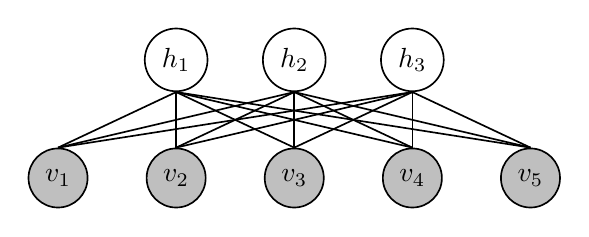
\begin{tikzpicture}[-,minimum size=0.75cm,node distance=1.5cm,semithick]
\tikzstyle{visible}=[circle,radius=1cm,fill=lightgray,draw=black,text=black,distance=1cm]
\tikzstyle{hidden}=[circle,radius=1cm,fill=white,draw=black,text=black,distance=1cm]
\node[visible] (v1)  [] {$v_1$};
\foreach \i in {2,3,4,5}
{
   \pgfmathtruncatemacro{\j}{\i-1};
   \node[visible] (v\i) [right of=v\j] {$v_{\i}$};
   \ifthenelse{\i<5}{\node[hidden]  (h\j) [above of=v\i] {$h_{\j}$}}{};
}
\foreach \i in {1,2,3,4,5}
   \foreach \j in {1,2,3}
      \path (v\i.north) edge (h\j.south);
\end{tikzpicture}
\end{center}

Energy of the RBM is given by
\BEQ
E(\hh,\vv) = -\aaa^T\vv - \bb^T\hh - \vv^T\Theta\hh = -\sum_{i} a_iv_i - \sum_j b_jh_j - \sum_{i,j} v_i\theta_{i,j}h_j.
\label{eq:Erbm}
\EEQ
Note that energy can be positive and negative in this setting, depending on the sign of the parameters $\aaa,\bb,\Theta$.

The distribution over states of this network
\BEQ
p(\hh,\vv|\Theta,\aaa,\bb) = \frac{\myexp{-E(\hh,\vv)}}{\sum_{\hh',\vv'} \myexp{-E(\hh',\vv')}} = \frac{\myexp{-E(\hh,\vv)}}{Z} \label{eq:prbm}
\EEQ

Several equations that will be helpful
\BEAN
\sum_{\hh,\vv} \frac{\myexp{-E(\hh,\vv)}f(\hh,\vv)}{\sum_{\hh',\vv'}\myexp{-E(\hh',\vv')}} &=& \sum_{\hh,\vv} p(\hh,\vv)f(\hh,\vv) \label{eq:energyprob}\\
\nabla \log \sum_{\hh,\vv} \myexp{-E(\hh,\vv)} &=& \frac{\sum_{\hh,\vv}\myexp{-E(\hh,\vv)}\nabla(-E(\hh,\vv))}{\sum_{\hh',\vv'}\myexp{-E(\hh',\vv')}} \nonumber \\
&=& \frac{\sum_{\hh,\vv}\myexp{-E(\hh,\vv)}\nabla(-E(\hh,\vv))}{Z} \nonumber \\
&=& \sum_{\hh,\vv} p(\hh,\vv) \nabla E(\hh,\vv) \label{eq:gradlogpartition} \\
\nabla \log \sum_{\hh} \myexp{-E(\hh,\vv)} &=& \frac{\sum_{\hh}\myexp{-E(\hh,\vv)}\nabla(-E(\hh,\vv))}{\sum_{\hh'}\myexp{-E(\hh',\vv)}} \nonumber \\
&=& \frac{\frac{\sum_{\hh}\myexp{-E(\hh,\vv)}}{Z}\nabla(-E(\hh,\vv))}{\frac{\sum_{\hh'}\myexp{-E(\hh',\vv)}}{Z}} \nonumber \\
&=&\frac{\sum_{\hh}p(\hh,\vv)\nabla(-E(\hh,\vv))}{\sum_{\hh'}p(\hh',\vv)} \nonumber \\
&=&\frac{\sum_{\hh}p(\hh,\vv)\nabla(-E(\hh,\vv))}{p(\vv)} \nonumber \\
&=&  \sum_{\hh} p(\hh|\vv) \nabla(-E(\hh,\vv)) \label{eq:gradlogmarginal}
\EEAN



\newproblem{2pt} We will use the bipartite structure of the graph to show that each $h_j$ is independent of the rest given $\vv$.
Specifically, we will show
\[
p(h_k | \vv, \hh_{[-k]},\Theta,\aaa,\bb) = p(h_k | \vv,\theta_{:,k},\bb)
\]
We will use the fully expanded energy:
\[
E(\hh,\vv) = -\left(\sum_{i} a_iv_i\right) - \left(\sum_j b_jh_j\right) - \sum_{i,j} v_i\theta_{i,j}h_j
\]
Organize the terms of the negative energy into those that depend on $h_k$ and those that do not
\BEAN
-E(\hh,\vv) &=& f(h_k,\vv) + g(\hh_{[-k]},\vv)  \label{eq:Efg} \\
f(h_k,\vv) &=& ... \label{eq:Ef}\\
g(\hh_{[-k]},\vv) &=& ...  \label{eq:Eg}
\EEAN
Using Equations~\ref{eq:prbm} and \ref{eq:Efg}, express $p(\hh,\vv)$ using $f$ and $g$. You can leave denominator as $Z$.
\BEQ
p(\hh,\vv) = ...
\label{eq:fgZ}
\EEQ
Use Bayes' rule, Equation~\ref{eq:bayes}, to express $p(h_k|\vv)$ in terms of $p(h_k,\vv)$ and $p(\vv)$
\BEQ
p(h_k | \vv) = ... \label{eq:conditional}
\EEQ
Express $p(h_k,\vv)$ using Equations~\ref{eq:split},\ref{eq:marg}. Then use Equation~\ref{eq:fgZ} and ~\ref{eq:distsimple}
\BEQ
p(h_k,\vv) = ... \label{eq:joint}
\EEQ
Express $p(\vv)$ by marginalizing out $\hh$ of $p(\hh,\vv)$,  then expand $p(\hh,\vv)$  using Equation~\ref{eq:fgZ}
\[
p(\vv) = ...
\]
Use Equation~\ref{eq:dist} to reorganize $p(\vv)$
\BEQ
p(\vv) = ...
\label{eq:marginal}
\EEQ
Use Equation~\ref{eq:conditional},~\ref{eq:joint},~\ref{eq:marginal} to express conditional probability
\[
p(h_k|\vv) = ...
\]

Cancel out terms and expand $f(h_k)$
\[
p(h_k|\vv) = ...
\]
Use the fact that $h_k \in \{0,1\}$ and write out this conditional probability as a sigmoid
\BEQ
p(h_k|\vv) = ...
\label{eq:conditionalsigmoid}
\EEQ
where
\[
\sigmoid{z} = \frac{1}{1 + \myexp{-z}}
\]

Use the fact that the energy has a symmetric form for visible and hidden variables and obtain conditional probability
\[
p(v_l | \hh) = ...
\]
Note that $\Theta$ is not symmetric, $\theta_{i,j} \neq \theta_{j,i}$ in fact $\Theta$ will usually have less columns than rows, since the hidden variables compress information in the visible ones.

\newproblem{2pt}

Implement sampling of conditional distribution given by Equation~\ref{eq:conditionalsigmoid}.
As input you will be provided $\Theta$ matrix with $m$ rows and $n$ columns, vector of biases $\cc$, and a vector of variables $\vv$.
Your code should sample all of the hidden variables at once. Note that the hidden variables are independent from each other given the visible variables. You proved this in the last problem.
\begin{verbatim}
function h = sample(Theta,cc,vv)
nvisible = size(Theta,1);
nhidden = size(Theta,2);
nsamples = size(vv,2);
assert(size(cc,1) == nvisible);
assert(size(vv,1) == nhidden);
zz = ... + repmat(...,[1 nsamples]);

h = sigmoid(zz) > rand(size(Theta,1),nsamples);

function p = sigmoid(zz)
p = 1./(1 + exp(-zz));
\end{verbatim}



\begin{center}
  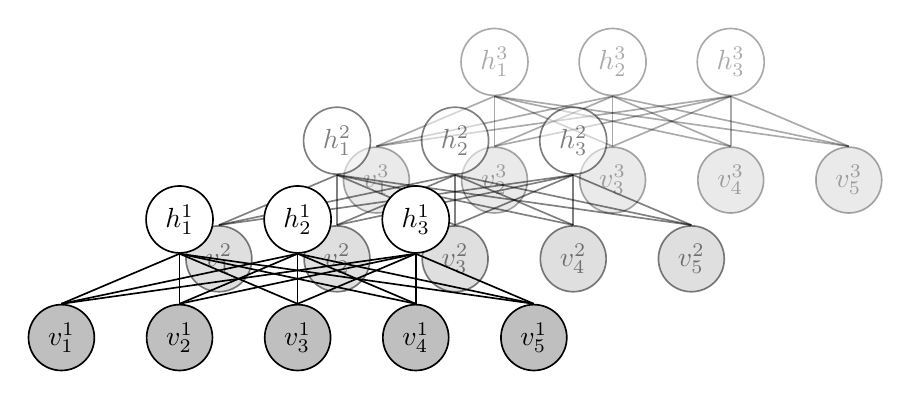
\begin{tikzpicture}[-,minimum size=0.75cm,node distance=1.5cm,semithick]
\tikzstyle{visible}=[circle,radius=1cm,fill=lightgray,draw=black,text=black,distance=1cm]
\tikzstyle{hidden}=[circle,radius=1cm,fill=white,draw=black,text=black,distance=1cm]

\foreach \d in {3,2,1}
{
\begin{scope}[shift=({2*\d,\d}),opacity=1/\d]
\node[visible] (v\d1)  [] {$v^{\d}_1$};

\foreach \i in {2,3,4,5}
{
   \pgfmathtruncatemacro{\j}{\i-1};
   \node[visible] (v\d\i) [right of=v\d\j] {$v^{\d}_{\i}$};
   \ifthenelse{\i<5}{\node[hidden]  (h\d\j) [above of=v\d\i] {$h^{\d}_{\j}$}}{};
}
\foreach \i in {1,2,3,4,5}
   \foreach \j in {1,2,3}
      \path (v\d\i.north) edge (h\d\j.south);
\end{scope}
}
\end{tikzpicture}


\end{center}

The graph above shows an RBM on 3 samples. Your code should be able to sample states for all the hidden variables in all the samples in parallel.
Make sure that your code can take as an input a matrix $\Theta$,vector $\cc$ and a {\em matrix} $\VV$. The matrix $\VV$ is of size $p \times n$ where
$p$ is number of features in a sample, and $n$ is the number of samples. You should be able to use matrix multiplication and \verb|repmat| to achieve this.

Test your code by running this
\begin{verbatim}
    nv = 3;
    nh = 2;
    n = 100;
    Theta = [ -10 10; -10 -10; 10 -10];
    bb = [2;2];
    aa = [-5;+5;-5];
    hidden = rand(2,n)>0.5;
    visible = sample(Theta,aa,hidden);
    newhidden = sample(Theta',bb,visible);
    err = (sum(sum(newhidden ~= hidden))/prod(size(hidden)))
\end{verbatim}
You should see something like this
\begin{verbatim}
err =
    0.0450
\end{verbatim}
You can play with this code as well
\begin{verbatim}
hidden = rand(2,n)>0.5;
for it=1:1000
    visible = sample(Theta,aa,hidden);
    newhidden = sample(Theta',bb,visible);
    err = (sum(sum(newhidden ~= hidden))/prod(size(hidden)))
    hidden = newhidden;
end
hist([1 2]*hidden,[0:3])
\end{verbatim}
The code above iterates between drawing from $p(\hh|\vv,\Theta,\aaa,\bb)$ and $p(\vv|\hh,\Theta,\aaa,\bb)$.
This is an example of a block Gibbs sampler. It is called block, because we are updating blocks of variables at once.
As we iterate the chain, the sample $(\hh,\vv)$ gets closer to a draw from the distribution $p(\hh,\vv)$.

Thus, we can implement
\begin{itemize}
\item sampler for $p(\hh|\vv)$  as  \verb|hidden = sample(Theta',bb,visible);|
\item sampler for $p(\vv|\hh)$ as  \verb|visible = sample(Theta,aa,hidden);|
\item joint sampler for $p(\hh,\vv)$ by iterating
\begin{verbatim}
     hidden = sample(Theta',bb,visible);
     visible = sample(Theta,aa,hidden);
\end{verbatim}
\end{itemize}
\newproblem{2pt} \paragraph{Deriving contrastive divergence updates}
We will derive the maximum likelihood update from scratch.

The likelihood function for RBM for a parameter tuple $\Psi=(\Theta,\aaa,\bb)$:
\BEAS
\ALL(\Psi) &=& \sum_{t=1}^T \frac{1}{T}\log p(\vv^t|\Psi) = \sum_t \frac{1}{T}\log \sum_{\hh^t} p(\vv^t,\hh^t|\Psi)  \\
&=& \sum_t \frac{1}{T}\log \sum_{\hh^t} \frac{\myexp{-E(\vv^t,\hh^t)}}{\sum_{\vv'\hh'} \myexp{-E(\vv',\hh')}} \\
&=& \sum_t \frac{1}{T}\left[\log \sum_{\hh^t} \myexp{-E(\vv^t,\hh^t)} - \sum_{t=1}^T \log \sum_{\vv',\hh'} \myexp{-E(\vv',\hh')}\right] \\
&=& \sum_t \frac{1}{T}\left[\underbrace{\log \sum_{\hh^t} \myexp{-E(\vv^t,\hh^t)}}_{A^t(\Psi)} - \underbrace{\log \sum_{\vv',\hh'} \myexp{-E(\vv',\hh')}}_{B(\Psi)}\right]
\EEAS
Hence
\BEAN
\nabla_\Psi \ALL(\Psi) &=& \sum_{t=1}^T \frac{1}{T}\left[\nabla_\Psi A^t(\Psi) - B(\Psi)\right] \label{eq:ALLgrad}\\
A^t(\Psi) &=& \log \sum_{\hh^t} \myexp{-E(\vv^t,\hh^t)} \\
B(\Psi) &=& \log \sum_{\vv',\hh'} \myexp{-E(\vv',\hh')}
\EEAN

Use Equations~\ref{eq:energyprob} and \ref{eq:gradlogmarginal} to compute gradient of $A^t(\Psi)$
\BEAN
\nabla_\Psi A^t(\Psi) &=& ... \\
&=&  ... \\
&=& ...\label{eq:Agrad}
\EEAN
Use Equations~\ref{eq:energyprob} and \ref{eq:gradlogpartition} to compute gradient of $B(\Psi)$
\BEAS
\nabla_\Psi B(\Psi) &=& ... \\
&=& ... \\
&=& ... \label{eq:Bgrad}
\EEAS
Using Equations~\ref{eq:Erbm},\ref{eq:Agrad},\ref{eq:Bgrad} compute partial derivatives with respect to $\theta_{i,j}$,$a_i$, and $b_j$.
\BEAS
\partd{A^t(\Psi)}{\theta_{i,j}}  &=& ... \\
\partd{A^t(\Psi)}{a_i} &=& ... \\
\partd{A^t(\Psi)}{b_j} &=& ... \\
\partd{B(\Psi)}{\theta_{i,j}}  &=& ... \\
\partd{B(\Psi)}{a_i}  &=& ... \\
\partd{B(\Psi)}{b_j}  &=& ...\\
\partd{\ALL(\Psi)}{\theta_{i,j}}  &=& \sum_t \frac{1}{T}\left[...\right] \\
\partd{\ALL(\Psi)}{a_i}  &=& \sum_t \frac{1}{T}\left[...\right] \\
\partd{\ALL(\Psi)}{b_i}  &=& \sum_t \frac{1}{T}\left[...\right]
\EEAS
\newproblem{2pt} Implement contrastive divergence for gradient computation

\begin{center}
\begin{algorithm}[H]
\DontPrintSemicolon
\SetCommentSty{textsf}
\SetKwComment{tcc}{}{}
\SetKwInOut{Input}{input}
\SetKwInOut{Output}{output}
\Input{$\Theta,\aaa,\bb,\{ \vv^t:t=1,\dots T\}$}
\Output{approximate gradient $\bg$ and recon}
recon = 0;
\ForEach{$t=1,2,\dots T$}{
Sample $\hh^t$ from $p(\hh|\vv^t,\Theta,\aaa,\bb)$\;
$\bg_{\theta}^0 = \bg_{\theta}^0 + \frac{1}{T}\answer$;
$\bg_{\aaa}^0 = \bg_{\aaa}^0 + \frac{1}{T}\answer$\;
$\bg_{\bb}^0 = \bg_{\bb}^0 + \frac{1}{T}\answer$\;
Sample $\vv^{t,1}$ from $p(\vv|\hh^t,\Theta,\aaa,\bb)$ \;
Sample $\hh^{t,1}$ from $p(\hh|\vv^{t,1},\Theta,\aaa,\bb)$ \;
$\bg_{\theta}^1 =  \bg_{\theta}^1 + \frac{1}{T}\answer$\;
$\bg_{\aaa}^1 = \bg_{\aaa}^1 + \frac{1}{T}\answer$\;
$\bg_{\bb}^1 = \bg_{\bb}^1 + \frac{1}{T}\answer$\;
recon = recon + err($\vv^t$,$\vv^{t,1}$)
}
$\bg = -\bg^0 + \bg^1$\;
\end{algorithm}
\end{center}
Note that computation for different $t=1,...,T$ can be performed in parallel.
Hence \verb|foreach| above is parallelizable.

\begin{verbatim}
function [bg_theta,bg_aa,bg_bb,recon] = cdgradient(Theta,aa,bb,V)
p = size(V,1);
T = size(V,2);
nhidden = size(Theta,2);
nvisible = size(Theta,1);
assert(length(aa) == nvisible)
assert(length(bb) == nhidden)
bg0_theta = zeros(size(Theta));
bg1_theta = bg0_theta;
bg0_aa = zeros(size(aa));
bg1_aa = bg0_aa;
bg0_bb = zeros(size(bb));
bg1_bb = bg0_bb;

recon = 0;
for t=1:T
    vt = V(:,t);
    ht = sample(Theta',bb,vt);
    bg0_theta = bg0_theta + ...;
    bg0_aa = bg0_aa + ...;
    bg0_bb = bg0_bb + ...;
    vt1 = sample(Theta,aa,ht);
    ht1 = sample(Theta',bb,vt1);
    bg1_theta = bg1_theta + ...;
    bg1_aa = bg1_aa + ...;
    bg1_bb = bg1_bb + ...;
    recon = recon + norm(vt1 - vt);
end
bg_theta = bg0_theta - bg1_theta;
bg_aa = bg0_aa - bg1_aa;
bg_bb = bg0_bb - bg1_bb;
\end{verbatim}




Try following code
\begin{verbatim}
nv = 3; nh = 2;
n = 100;
% ground truth params
Theta = [ -10 10; -10 -10; 10 -10];
bb = [2;2]; aa = [-5;+5;-5];

hidden = rand(nh,n)>0.5;

% sample from p(h,v)
for it=1:100
    visible = sample(Theta,aa,hidden);
    hidden = sample(Theta',bb,visible);
end

% step size
eta = 0.05;
% momentum
mom = 0.95;
% learned parameters
lTheta = 0.1*randn(size(Theta));laa = zeros(size(aa));lbb = zeros(size(bb));
% update direction
vt = zeros(size(Theta));vaa = zeros(size(aa));vbb = zeros(size(bb));
for it=1:10000
    [gt,ga,gb,recon] = cdgradient(lTheta,laa,lbb,visible);
    vaa = mom*vaa + eta*ga; vbb = mom*vbb + eta*gb; vt = mom*vt + eta*gt;
    lTheta = lTheta + vt; laa = laa + vaa; lbb = lbb + vbb;
    if (mod(it,100) == 0)
        fprintf('Iter: %d recon: %g ',it,recon);
        fprintf('Distance of learned theta to ground truth theta: %g\n',...
                min([norm(lTheta - Theta) norm(lTheta - Theta(:,[2 1]))]))
    end
end
\end{verbatim}

If you implemented \verb|cdgradient| correctly you should see the distance between the
learned theta \verb|lTheta| and ground truth theta used to generate data \verb|Theta| shrink.
Note that is might bounce around a bit in the later steps, since we are keeping a fixed
step size. You could try annealing the step size, \eg \verb|eta = 0.9999*eta|.

\newproblem{2pt}
We are going to train an RBM on digit images ... AND MAKE A MOVIE!
Download and decompress  MNIST training set from:

\url{http://yann.lecun.com/exdb/mnist/train-images-idx3-ubyte.gz}

Use following script to train your model
\begin{verbatim}
img = loadMNISTImages('train-images-idx3-ubyte');
lab = loadMNISTLabels('train-labels-idx1-ubyte');

nv = size(img,1);
nh = 100;
n = size(img,2);

% step size
eta = 0.1;
% momentum
mom = 0.95;
% learned parameters
lTheta = 0.1*randn(nv,nh);laa = zeros(nv,1);lbb = zeros(nh,1);
% update direction
vt = zeros(size(lTheta));vaa = zeros(size(laa));vbb = zeros(size(lbb));
minibatch = 100;
last = 0;
list = randperm(n);
ct = 0;
ITER = 1000;
d = sqrt(nv);
f = sqrt(nh);
skip = 10;
makemovie = 0;
if makemovie
    frames = zeros((d+1)*f+1,(d+1)*f+1,1,ceil(ITER/skip));
end

for it=1:ITER
    idxs = list(mod(last:last+minibatch-1,n)+1);
    last = last+minibatch;
    visible = img(:,idxs);
    eta = eta*0.9999;
    [gt,ga,gb,recon] = cdgradient(lTheta,laa,lbb,visible);
    vt = mom*vt + eta*gt;vaa = mom*vaa + eta*ga;vbb = mom*vbb + eta*gb;
    lTheta = lTheta + vt; laa = laa + vaa; lbb = lbb + vbb;
    if (mod(it,skip) == 0)
        fprintf('Iter: %d Recon: %d\n',it,recon);
        if makemovie
            ct = ct+1;
            frames(:,:,1,ct) = showfilters(lTheta);
        end
    end
end

if makemovie
    frames = frames(:,:,:,1:ct);
    frames = frames - min(frames(:));
    frames = frames./max(frames(:));
    frames = uint8(frames*255);
    mov = immovie(frames,gray(256));
    writerObj = VideoWriter('learning.mpg','MPEG-4')
    open(writerObj);
    writeVideo(writerObj,mov);
    close(writerObj);
end
\end{verbatim}
Tune the learning rate, \verb|eta|, momentum, \verb|mom|, minibatch size, \verb|minibatch|, so that
the filters looks like handwritten digits. Then switch the makemovie to be 1, rerun the code, and send the resulting video along with your homework report.

\end{document}
